\chapter{Lösungsdetails}
    \label{chapter:SolutionDetails}

    % Spezifikation zur Beschreibung von REST Schnittstellen: https://www.openapis.org/

    \section{Sprache zur Klassendefinition}
        \subsection{Sprachkonzepte}
            \begin{figure}
                \centering
                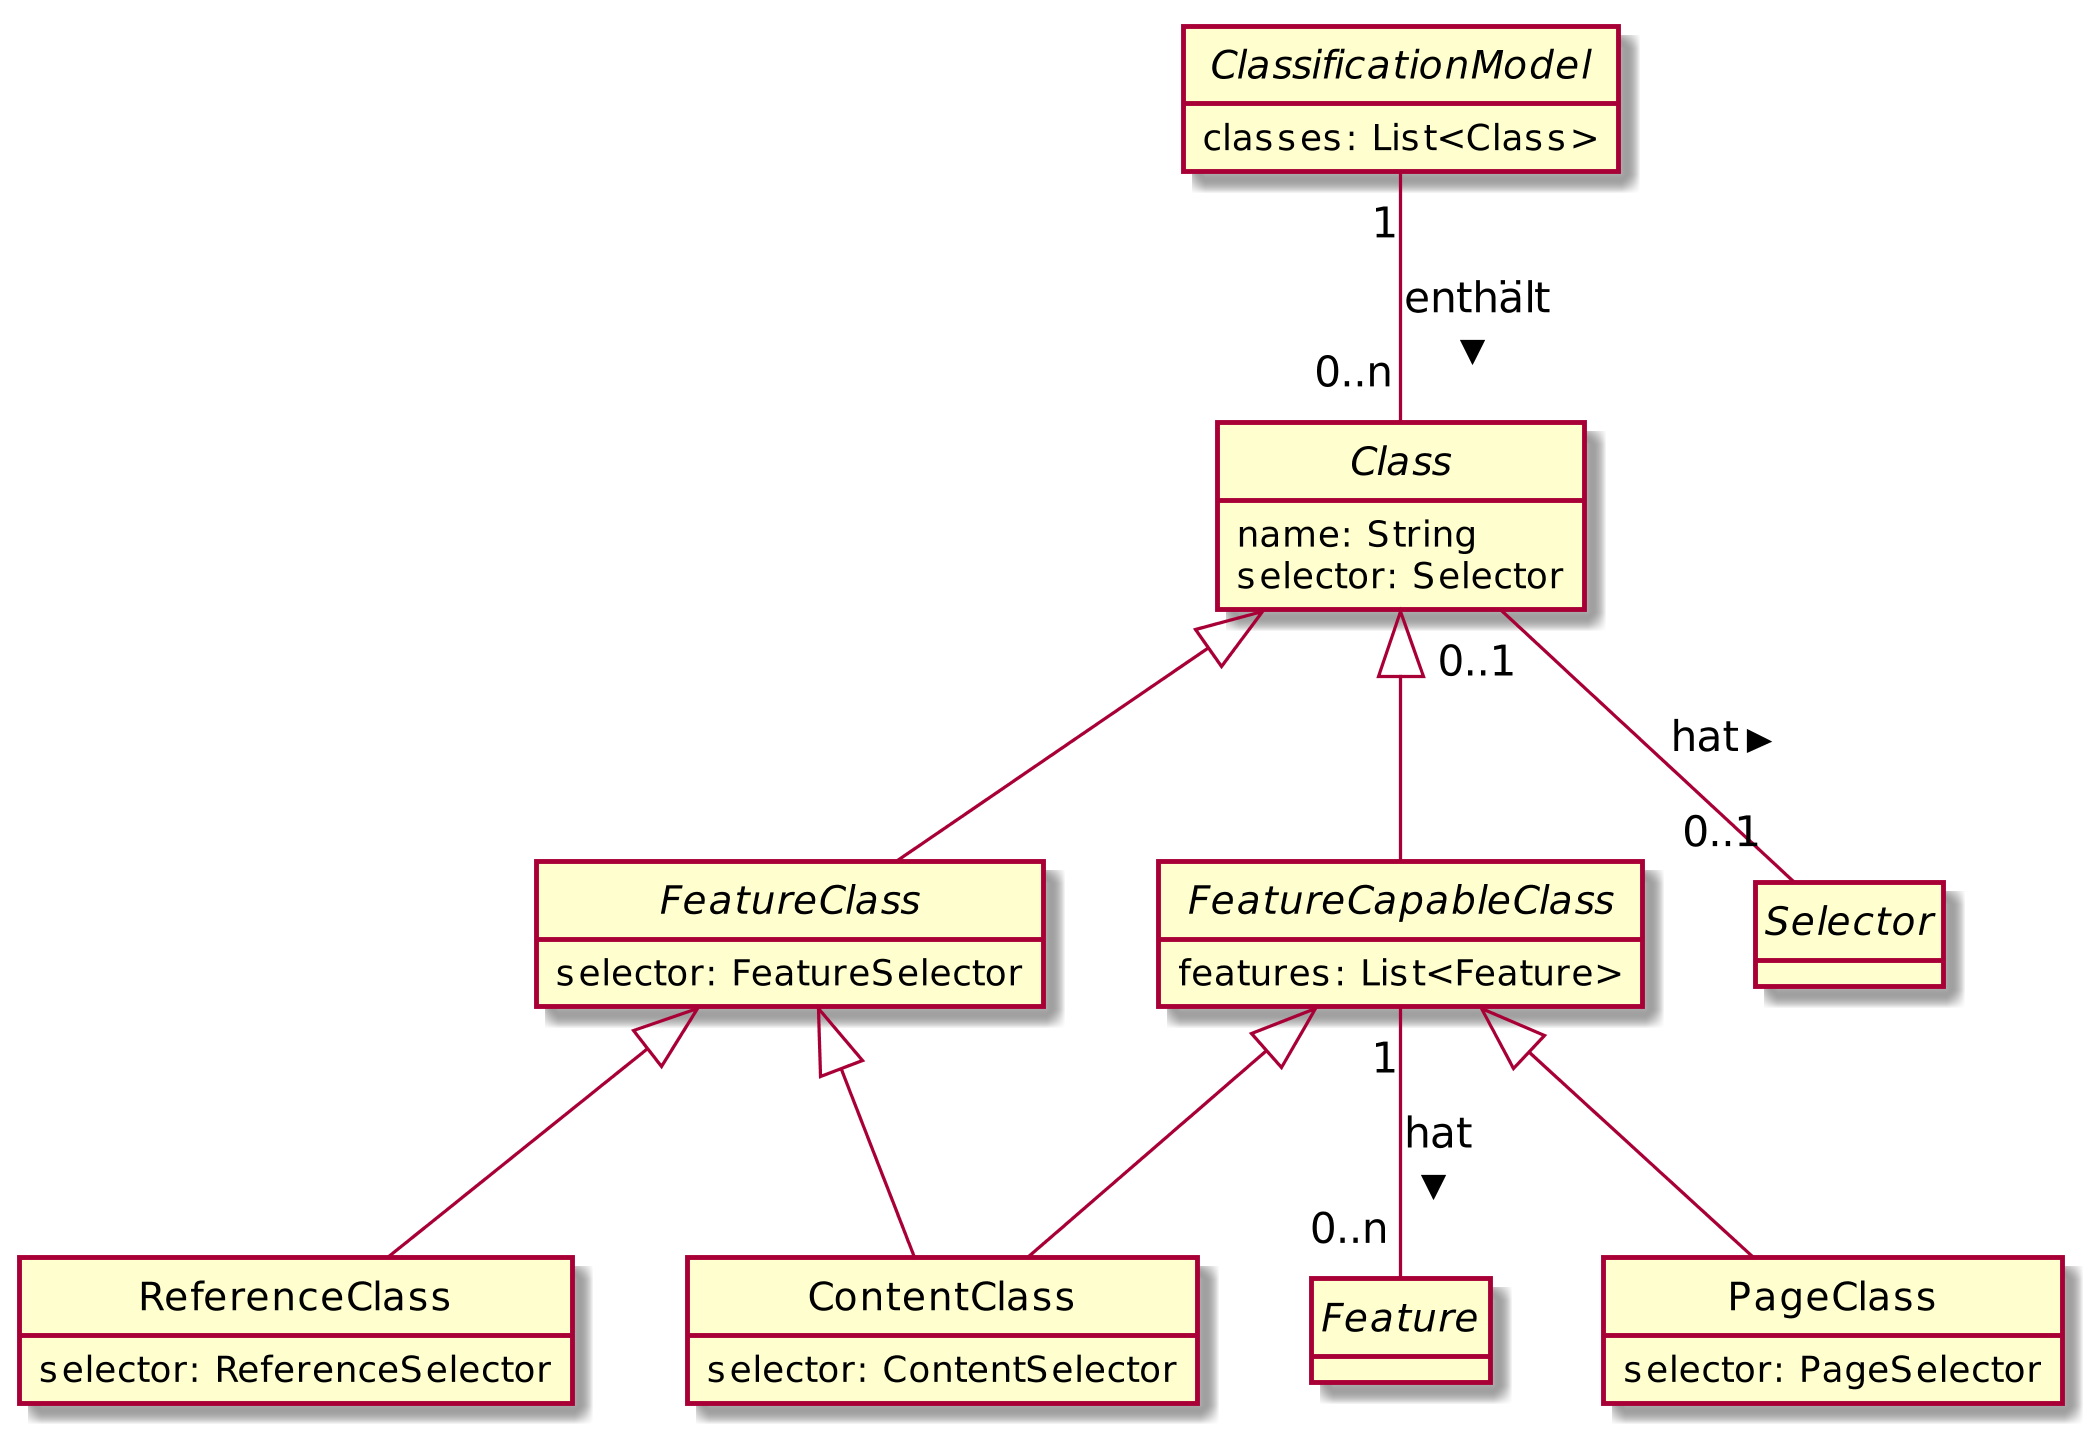
\includegraphics[width=\textwidth]{../resources/dsl/classes.png}
                \caption{Klassen in der DSL}
                \label{image:dslClasses}
            \end{figure}

            \begin{figure}
                \centering
                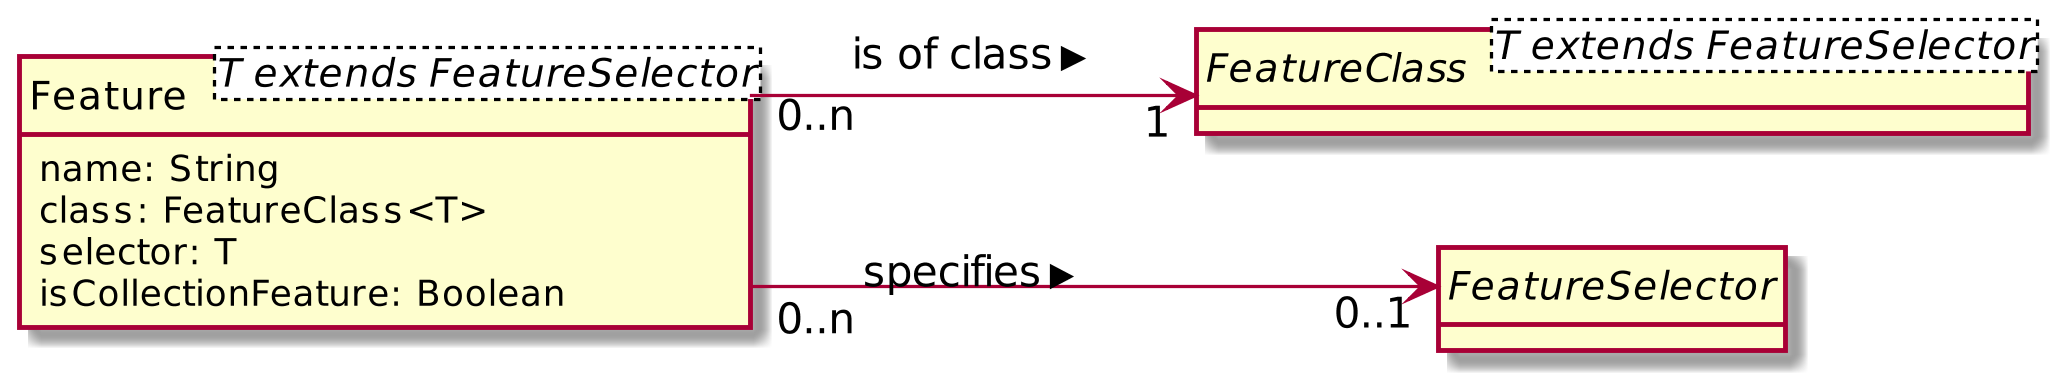
\includegraphics[width=\textwidth]{../resources/dsl/features.png}
                \caption{Features in der DSL}
                \label{image:dslFeatures}
            \end{figure}

            \begin{figure}
                \centering
                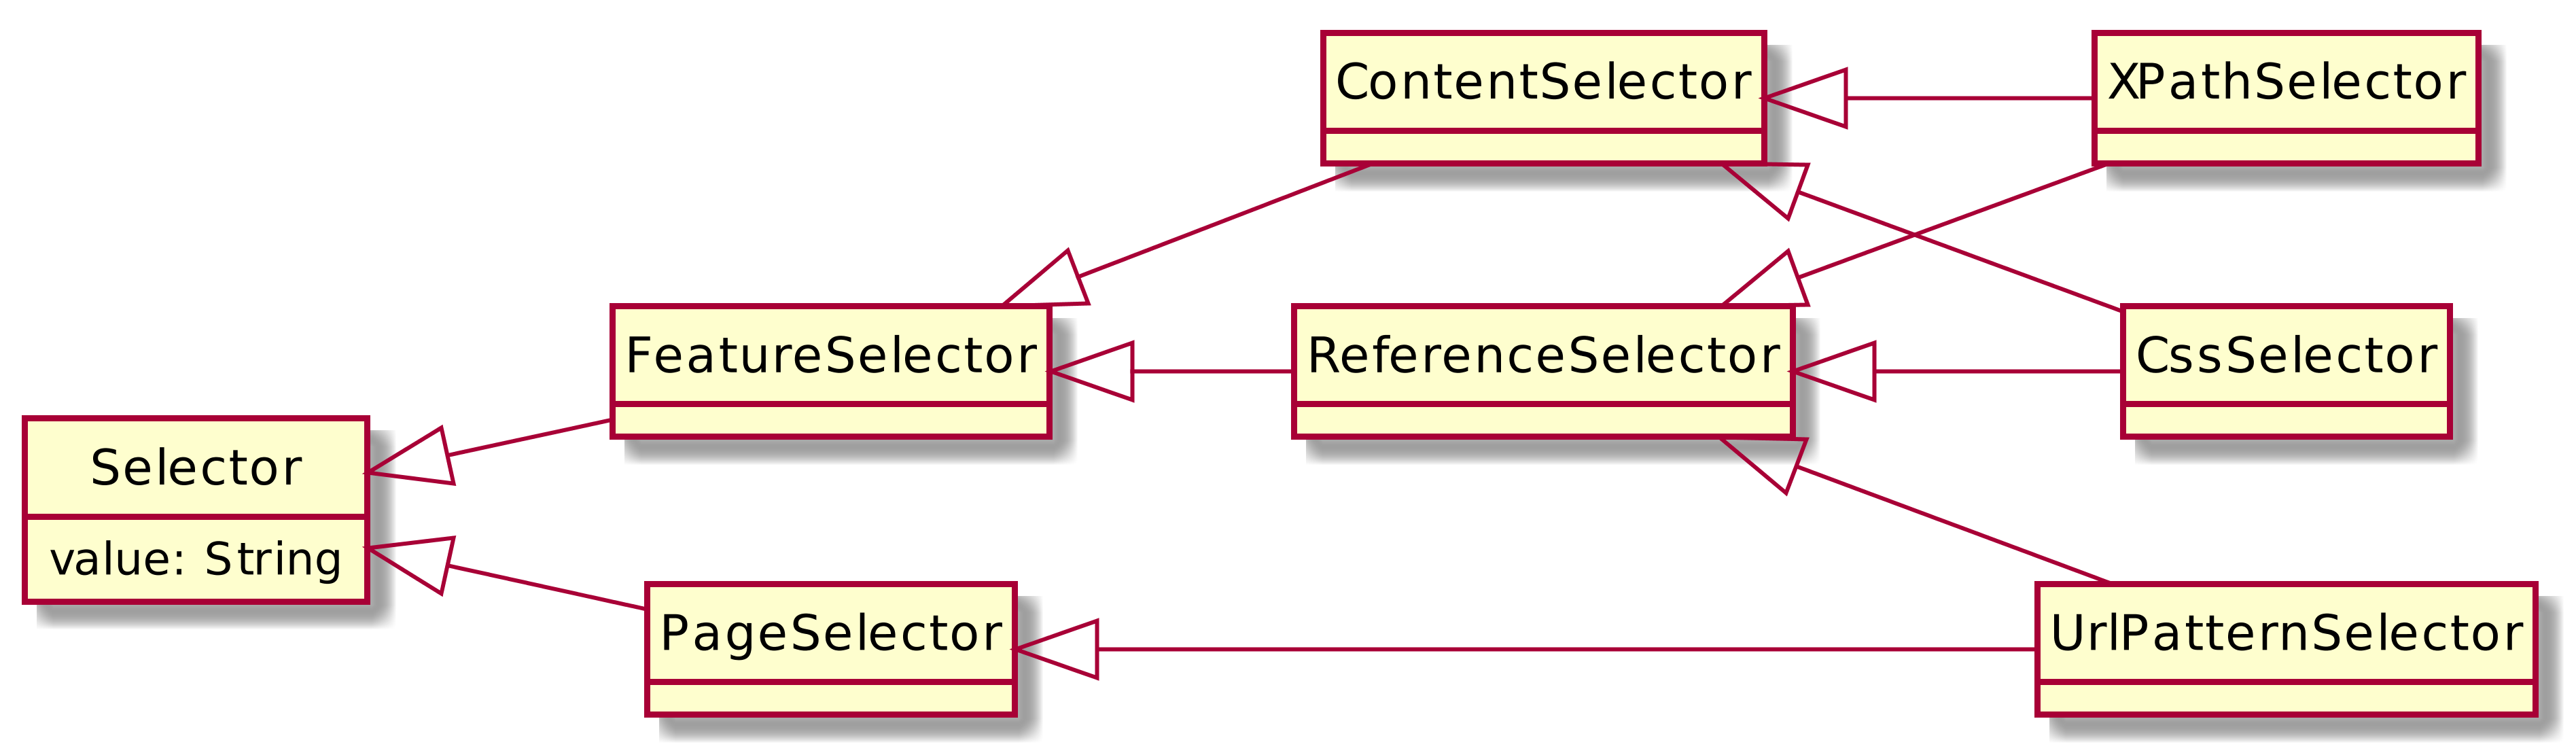
\includegraphics[width=\textwidth]{../resources/dsl/selectors.png}
                \caption{Selektoren in der DSL}
                \label{image:dslSelektoren}
            \end{figure}
            

    \section{Klassifizierungssystem}
    \section{Persistenz}
        \subsection{Classification Storage}
            Es wird eine Graphdatenbank verwendet!
        
        \subsection{Datenmodell}
            Wie sind die Daten in der DB modelliert?
        
            \begin{figure}
                \centering
                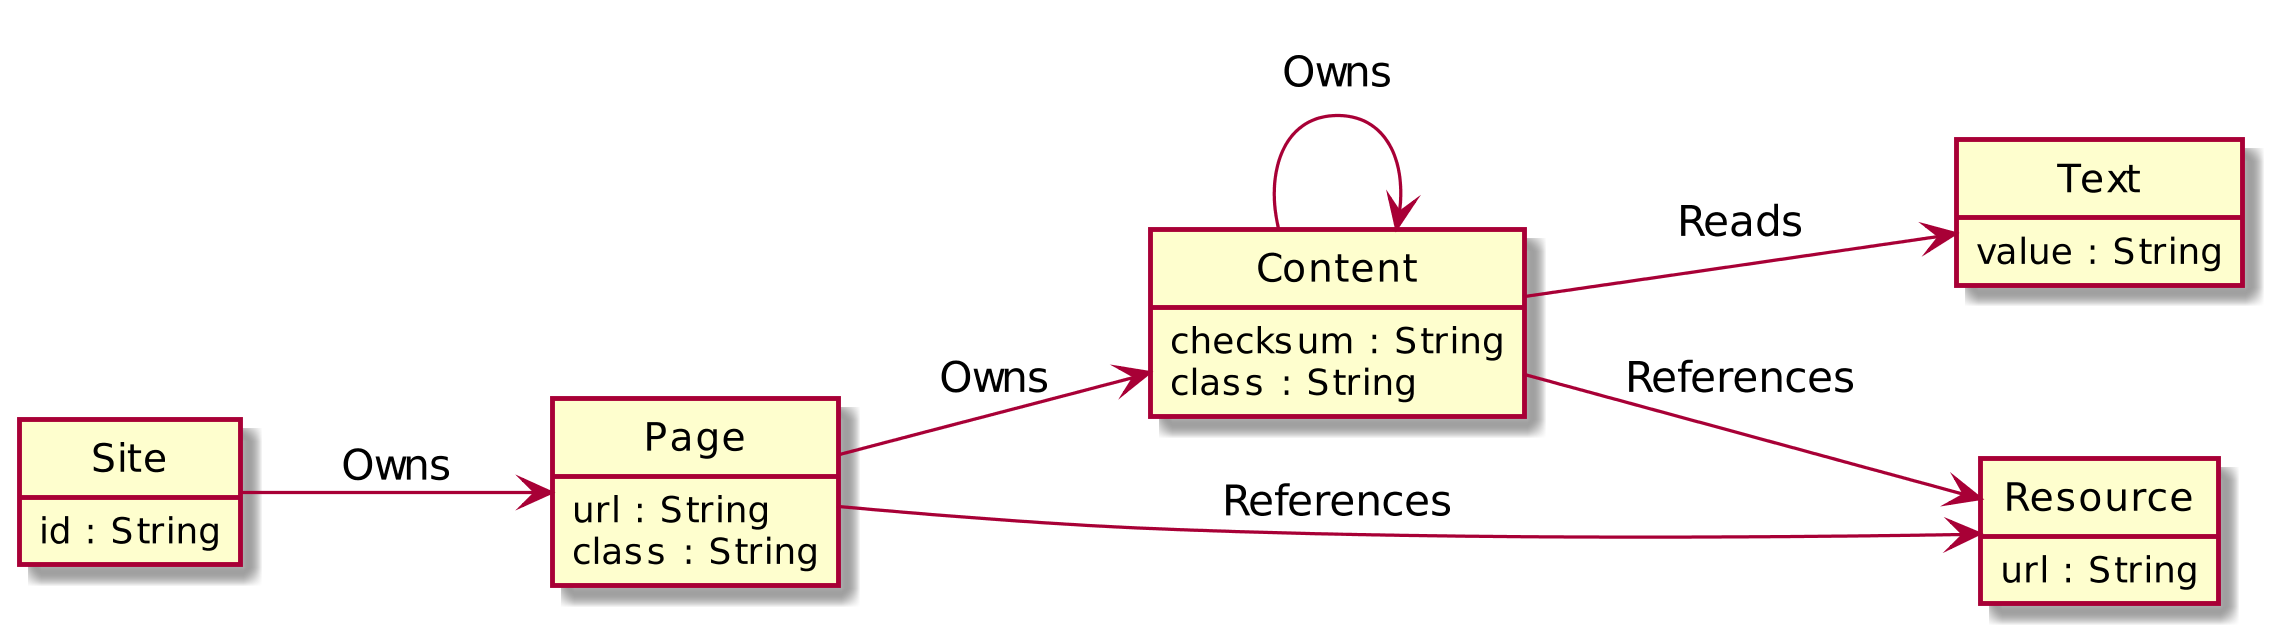
\includegraphics[width=\textwidth]{../resources/db-data-model/nodes.png}
                \caption{Übersicht der Nodes und ihrer Beziehungen}
                \label{image:dbDataModelOverview}
            \end{figure}

            \begin{figure}
                \centering
                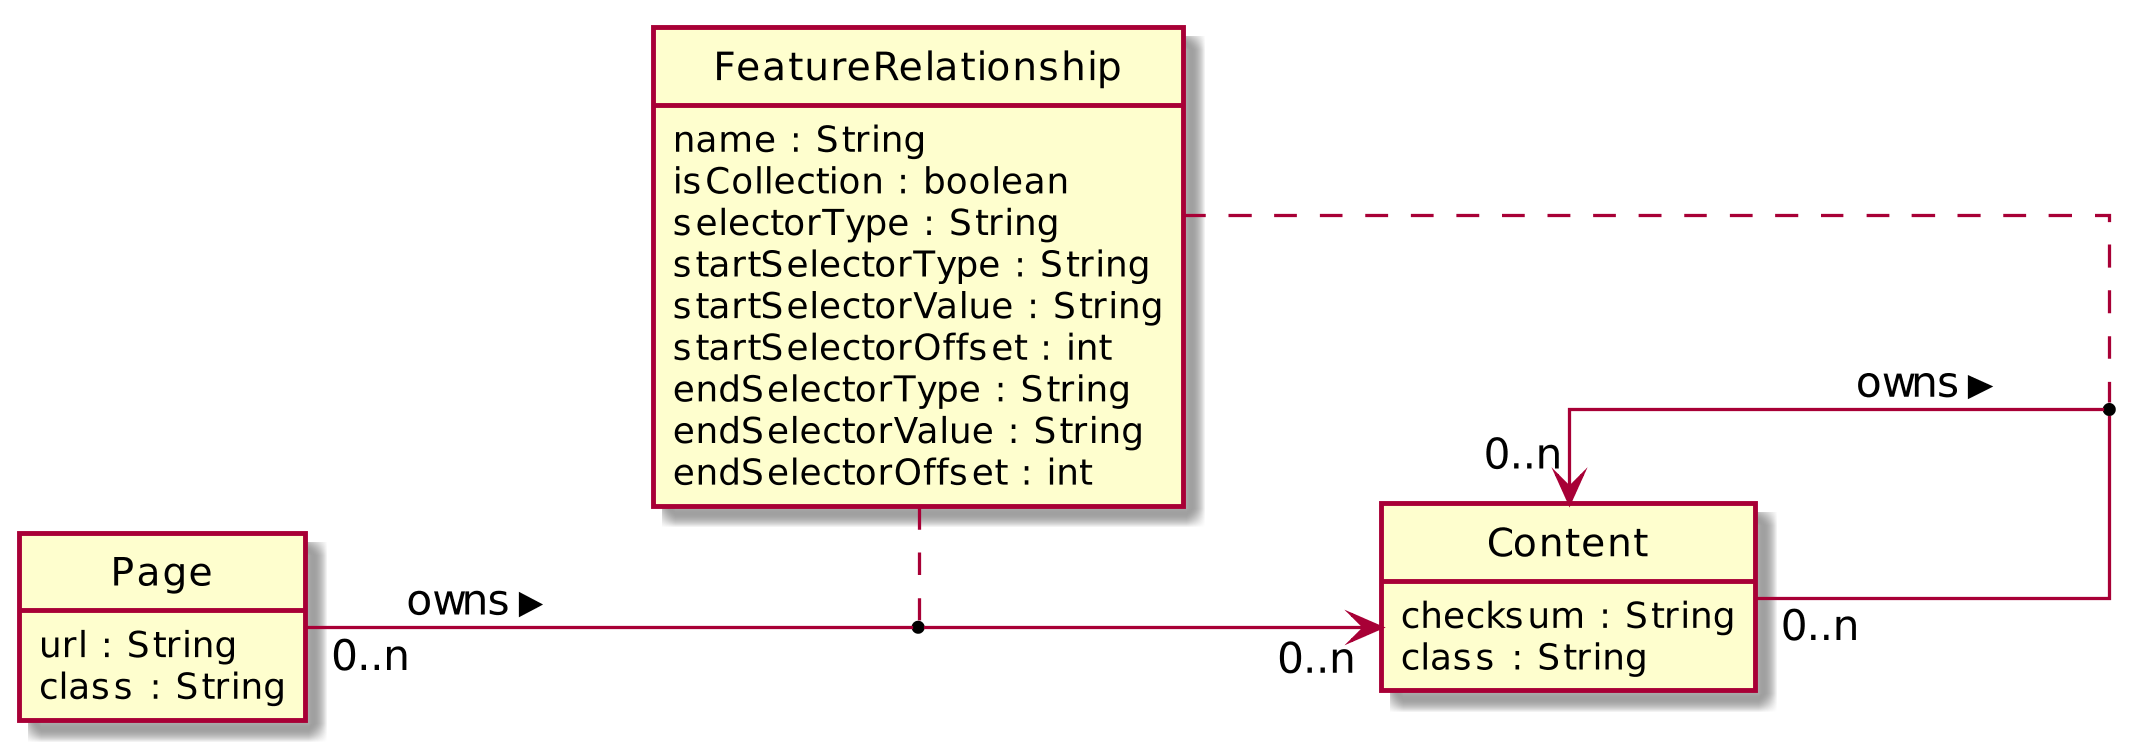
\includegraphics[width=\textwidth]{../resources/db-data-model/content-relationship.png}
                \caption{Content Features}
                \label{image:dbDataModelContentRelationship}
            \end{figure}

            \begin{figure}
                \centering
                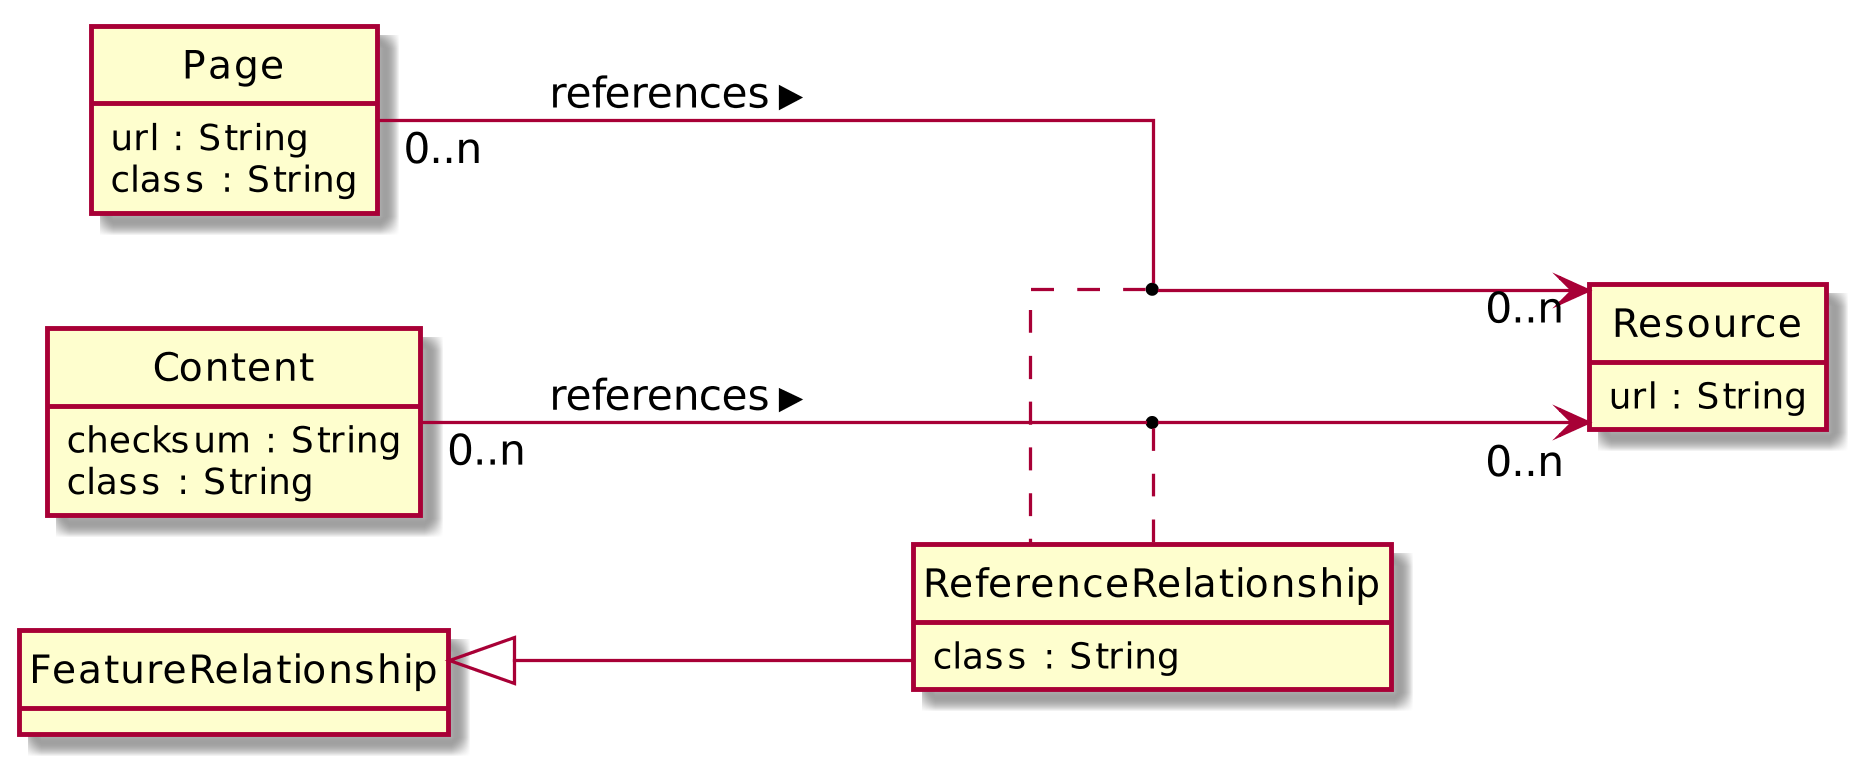
\includegraphics[width=\textwidth]{../resources/db-data-model/resource-relationship.png}
                \caption{Reference Features}
                \label{image:dbDataModelResourceRelationship}
            \end{figure}

        \subsection{Datenmodell Beispiel}
            \begin{figure}
                \centering
                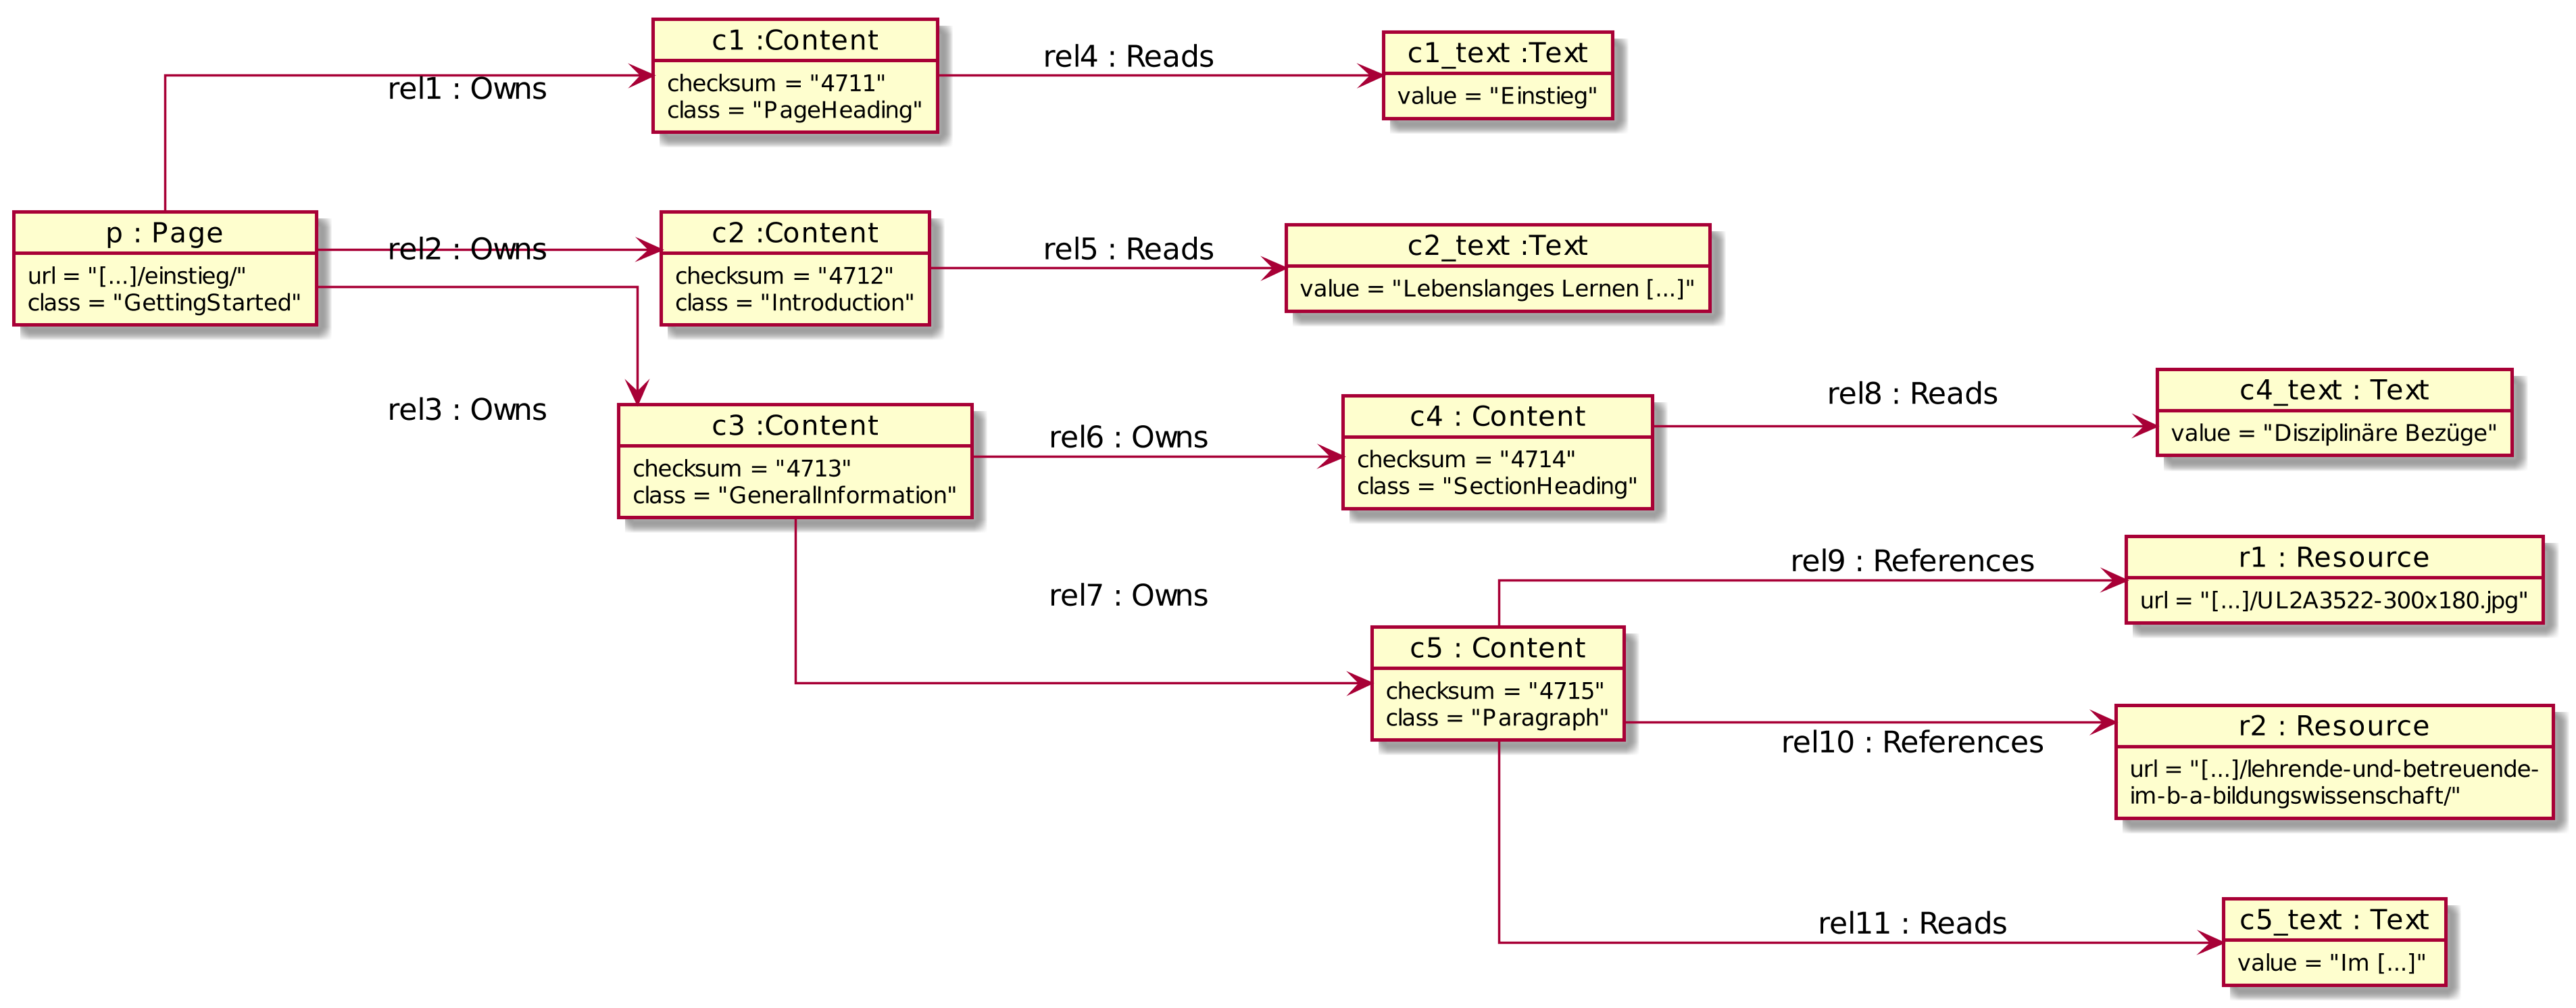
\includegraphics[width=\textwidth]{../resources/db-data-model/example/example.png}
                \caption{Beispiel}
                \label{image:dbDataModelExampleOverview}
            \end{figure}

            \begin{figure}
                \centering
                \begin{subfigure}{\textwidth}
                    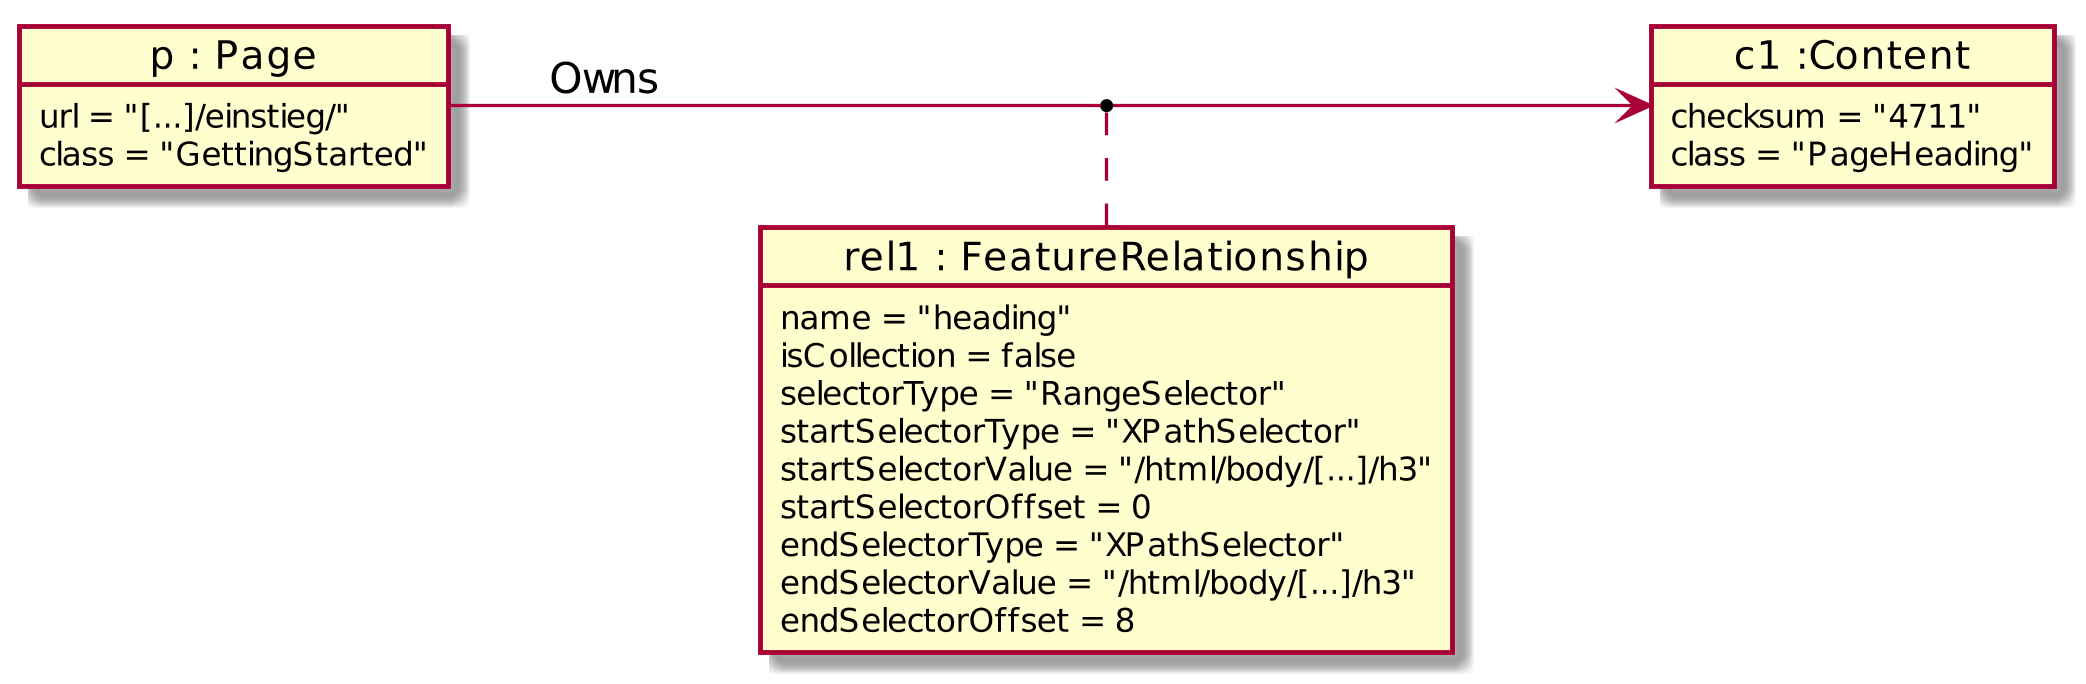
\includegraphics[width=\textwidth]{../resources/db-data-model/example/p-c1.png}
                    \subcaption{Rel 1}                    
                \end{subfigure}

                \begin{subfigure}{\textwidth}
                    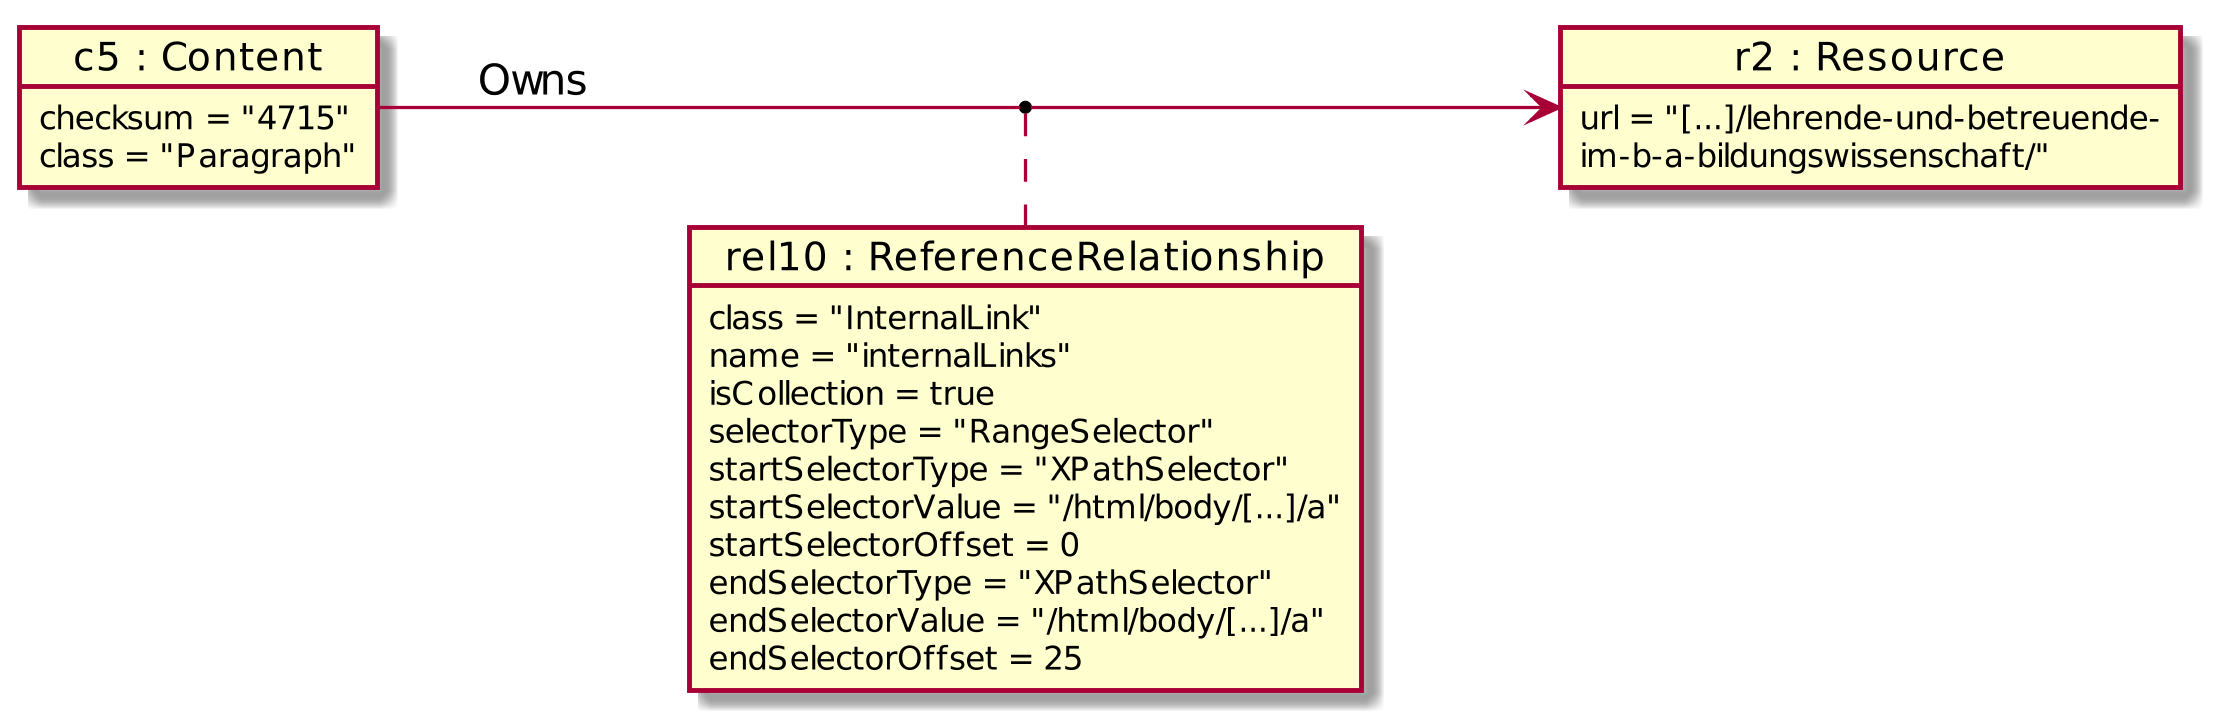
\includegraphics[width=\textwidth]{../resources/db-data-model/example/c5-r2.png}
                    \subcaption{Rel 2}                    
                \end{subfigure}
                \caption{Beziehungen}
                \label{image:dbDataModelExampleRelationships}
            \end{figure}

        \subsection{Classification Storage API}
            Wie werden die Daten in die DB geschrieben bzw. gelesen.

        \subsection{Was ist eine Seite}
            \begin{figure}
                \centering
                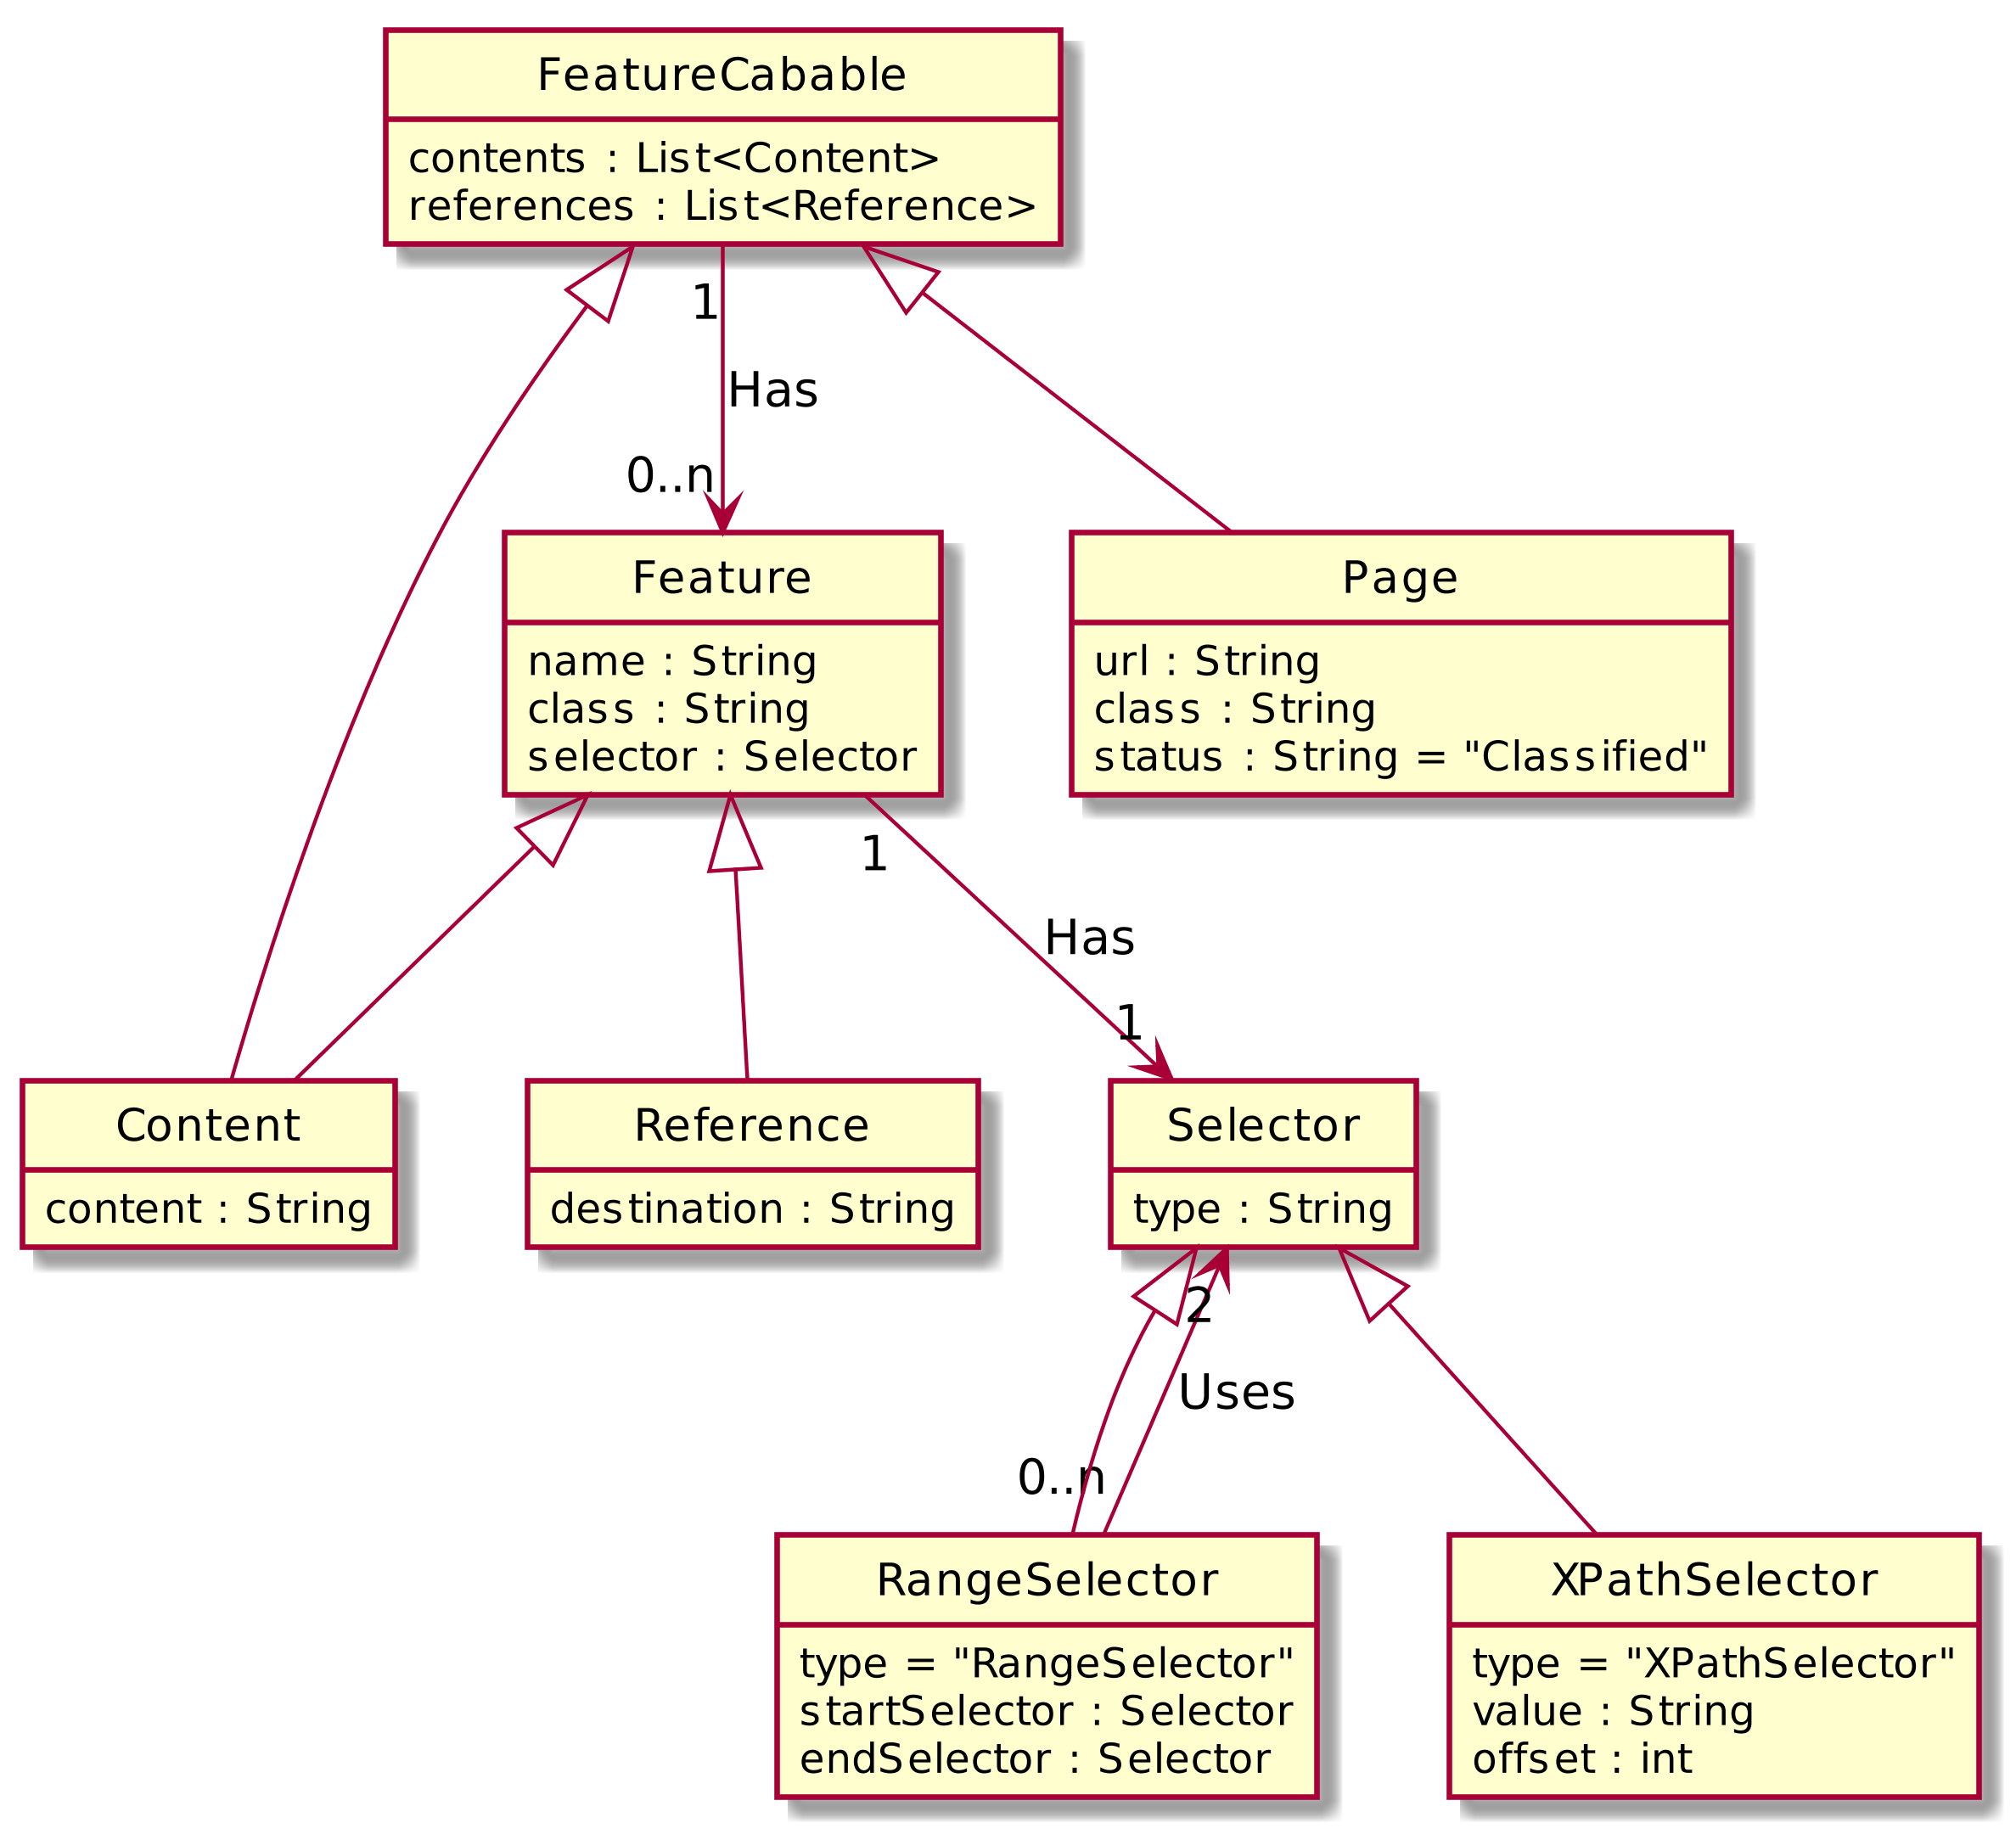
\includegraphics[width=\textwidth]{../resources/storage-api-data-model/page.png}
                \caption{Seite in der Storage API}
                \label{image:storageApiPageModel}
            \end{figure}
        
        \subsection{Algorithmus zum (initialen) ANLEGEN}
            \lstinputlisting[label=listing:storeClassification,caption=Algorithmus zum Speichern]{../resources/store-classification.code}

    \section{Annotation Service}
        \begin{table}[htb]
            \centering
            \begin{tabular}{|l|l|}
            \hline
            \textbf{Endpunkt}     & /pages/\{pageId\}\\
            \hline
            \textbf{Methode}      & GET\\
            \hline
            \textbf{Beschreibung} & Liefert Annotator Storage API version\\
            \hline
            \textbf{Status}       & 200\\
            \hline
            \textbf{Antwort}      & \{ ``name'': ``Annotator Store API'', ``version'': ``2.0.0'' \}\\
            \hline
            & \\
            \hline
            \textbf{Endpunkt}     & /pages/\{pageId\}/annotations\\
            \hline
            \textbf{Methode}      & GET\\
            \hline
            \textbf{Beschreibung} & Liefert alle Annotationen einer Seite\\
            \hline
            \textbf{Status}       & 200\\
            \hline
            \textbf{Antwort}      & \{ ``name'': ``Annotator Store API'', ``version'': ``2.0.0'' \}\\
            \hline
            \end{tabular}
            \caption{My caption}
            \label{my-label}
        \end{table}
        % Schnittstellenbeschreibung:
        % - Endpunkt
        % - Methoden
        % -- Input-Dokument
        % -- Status Codes der Antwort
        % -- Return Dokument für jede Antwort

    \section{Annotator Plugin}
    \section{Webanwendung}
    \section{WordPress Crawler}

    